\chapter{Human Intention and Motion Prediction Framework}
\label{chap:framework}

%----------------------------------------------------------------------------------------
\section{Introduction}
%----------------------------------------------------------------------------------------

The paradigm of Digital Twins has found widespread application in optimizing performance across diverse industrial sectors, including manufacturing, aerospace, and energy \citep{Andronas2021, Polini2020}. However, conventional digital twins often prioritize technical system aspects, frequently overlooking the human element crucial for Industry 5.0. Human-Centric Digital Twins (HCDTs) aim to address this by integrating models of human behavior, cognition, and even emotion, thereby enabling personalized and adaptive feedback to human operators \citep{Usman}. A truly effective HCDT allows the predicted intention and motion to be utilized in several ways: for real-time monitoring of operator performance, for providing semantic assistance, such as prompting the operator on the next step or flagging procedural errors, and for enabling a robotic assistant to proactively provide physical support.

Such HCDTs promise to elevate safety, efficiency, and productivity in human-machine systems, while concurrently enhancing user experience and satisfaction \citep{Umbrico2022}. In high-mix, low-volume (HMLV) industrial contexts, traditional automation systems exhibit significant rigidity, necessitating substantial human intervention for customization and adaptation. The advent of Machine Learning (ML), Artificial Intelligence (AI), and advanced automation technologies offers a pathway towards more flexible solutions, particularly beneficial for Small and Medium Enterprises (SMEs). These innovations can facilitate partial automation of labor-intensive tasks or enable collaborative human-robot workflows, where humans focus on complex reasoning and dexterous manipulation, while robots manage repetitive actions \citep{Cotta2023, Sirintuna2024}.

Current AI systems are approaching a semantic understanding of human actions and intentions, but translating this understanding into accurate 3D motion prediction remains an open problem. This predictive capability is paramount for robots to transition from reactive assistance to smart collaboration. To address this challenge, this chapter presents a modular and scalable framework that utilizes Vision-Language Models (VLMs) with motion diffusion techniques to predict human intent and generate plausible future human motion in semi-structured environments.

\subsection{Motivation for a Modular Approach}

Instead of pursuing end-to-end training, the approach presented in this thesis emphasizes the integration of existing, pre-trained perception and reasoning modules. This design philosophy not only makes the system more practical for SMEs with limited computational resources and training data, who can benefit from leveraging pre-trained foundation models rather than training custom models from scratch, but also ensures adaptability, as overall framework performance can improve with advancements in individual modules without requiring complete system re-training. The modular design further allows for inspection and debugging of intermediate outputs, facilitating understanding of system behavior and failure modes, and different modules can be swapped or upgraded independently based on application requirements or available computational resources.

This modular philosophy directly addresses the limitations identified in Chapter~\ref{chap:literature}, where existing approaches either focus narrowly on action recognition within limited classes or produce context-agnostic pose forecasts that fail to account for task semantics and environmental constraints.

\subsection{Chapter Overview}

The remainder of this chapter is organized as follows. Section~\ref{sec:framework_architecture} presents the high-level architecture of the proposed framework, introducing its three primary modules and their interconnections. Section~\ref{sec:perception_scene} details the Perception and Scene Representation module, covering human pose estimation, 3D scene grounding, and gaze analysis. Section~\ref{sec:ai_reasoning} describes the AI-Driven Reasoning and Intent Prediction module, including task knowledge representation and the two-phase prediction pipeline. Section~\ref{sec:motion_generation} presents the Human Motion Generation module, which synthesizes physically plausible 3D motion from predicted intent. Finally, Section~\ref{sec:chapter_summary} summarizes the key contributions of the proposed framework.

%----------------------------------------------------------------------------------------
\section{Proposed Framework Architecture}
\label{sec:framework_architecture}
%----------------------------------------------------------------------------------------

A modular framework is proposed to enable intelligent Human-Robot Collaboration (HRC) by predicting human intention and future pose. This methodology is designed to bridge the gap between short-term motion forecasting and long-term action planning, ensuring predictions are both physically plausible and contextually appropriate.

\subsection{High-Level Overview}

Formally, the predictive challenge is to process a stream of multimodal data to predict human intention and motion. Let the input at any given time $t$ consist of a history of video frames $\mathcal{V} = \{I_k\}_{k=1}^t$, extracted human poses $\mathcal{P} = \{P_k\}_{k=1}^t$, and static, high-level task knowledge $\mathcal{C}_{task}$. The framework, represented by a function $\mathcal{F}$, processes this context to give three outputs: the predicted task state $S_t$, which captures the current progress within the overall workflow; a forecast of future hand positions $\hat{H}_{t+\Delta t} = ( (x_l, y_l), (x_r, y_r) )$, for a time horizon $\Delta t$; and a full-body 3D motion trajectory $\hat{M}_{t_i} = \{\hat{x}_{t_i+1}, \ldots, \hat{x}_{t_i+N_{\text{pred}}}\}$.

The proposed framework, illustrated in Figure~\ref{fig:framework_overview}, has three primary modules that work in concert to achieve context-aware motion prediction.

\begin{figure}[htbp]
    \centering
    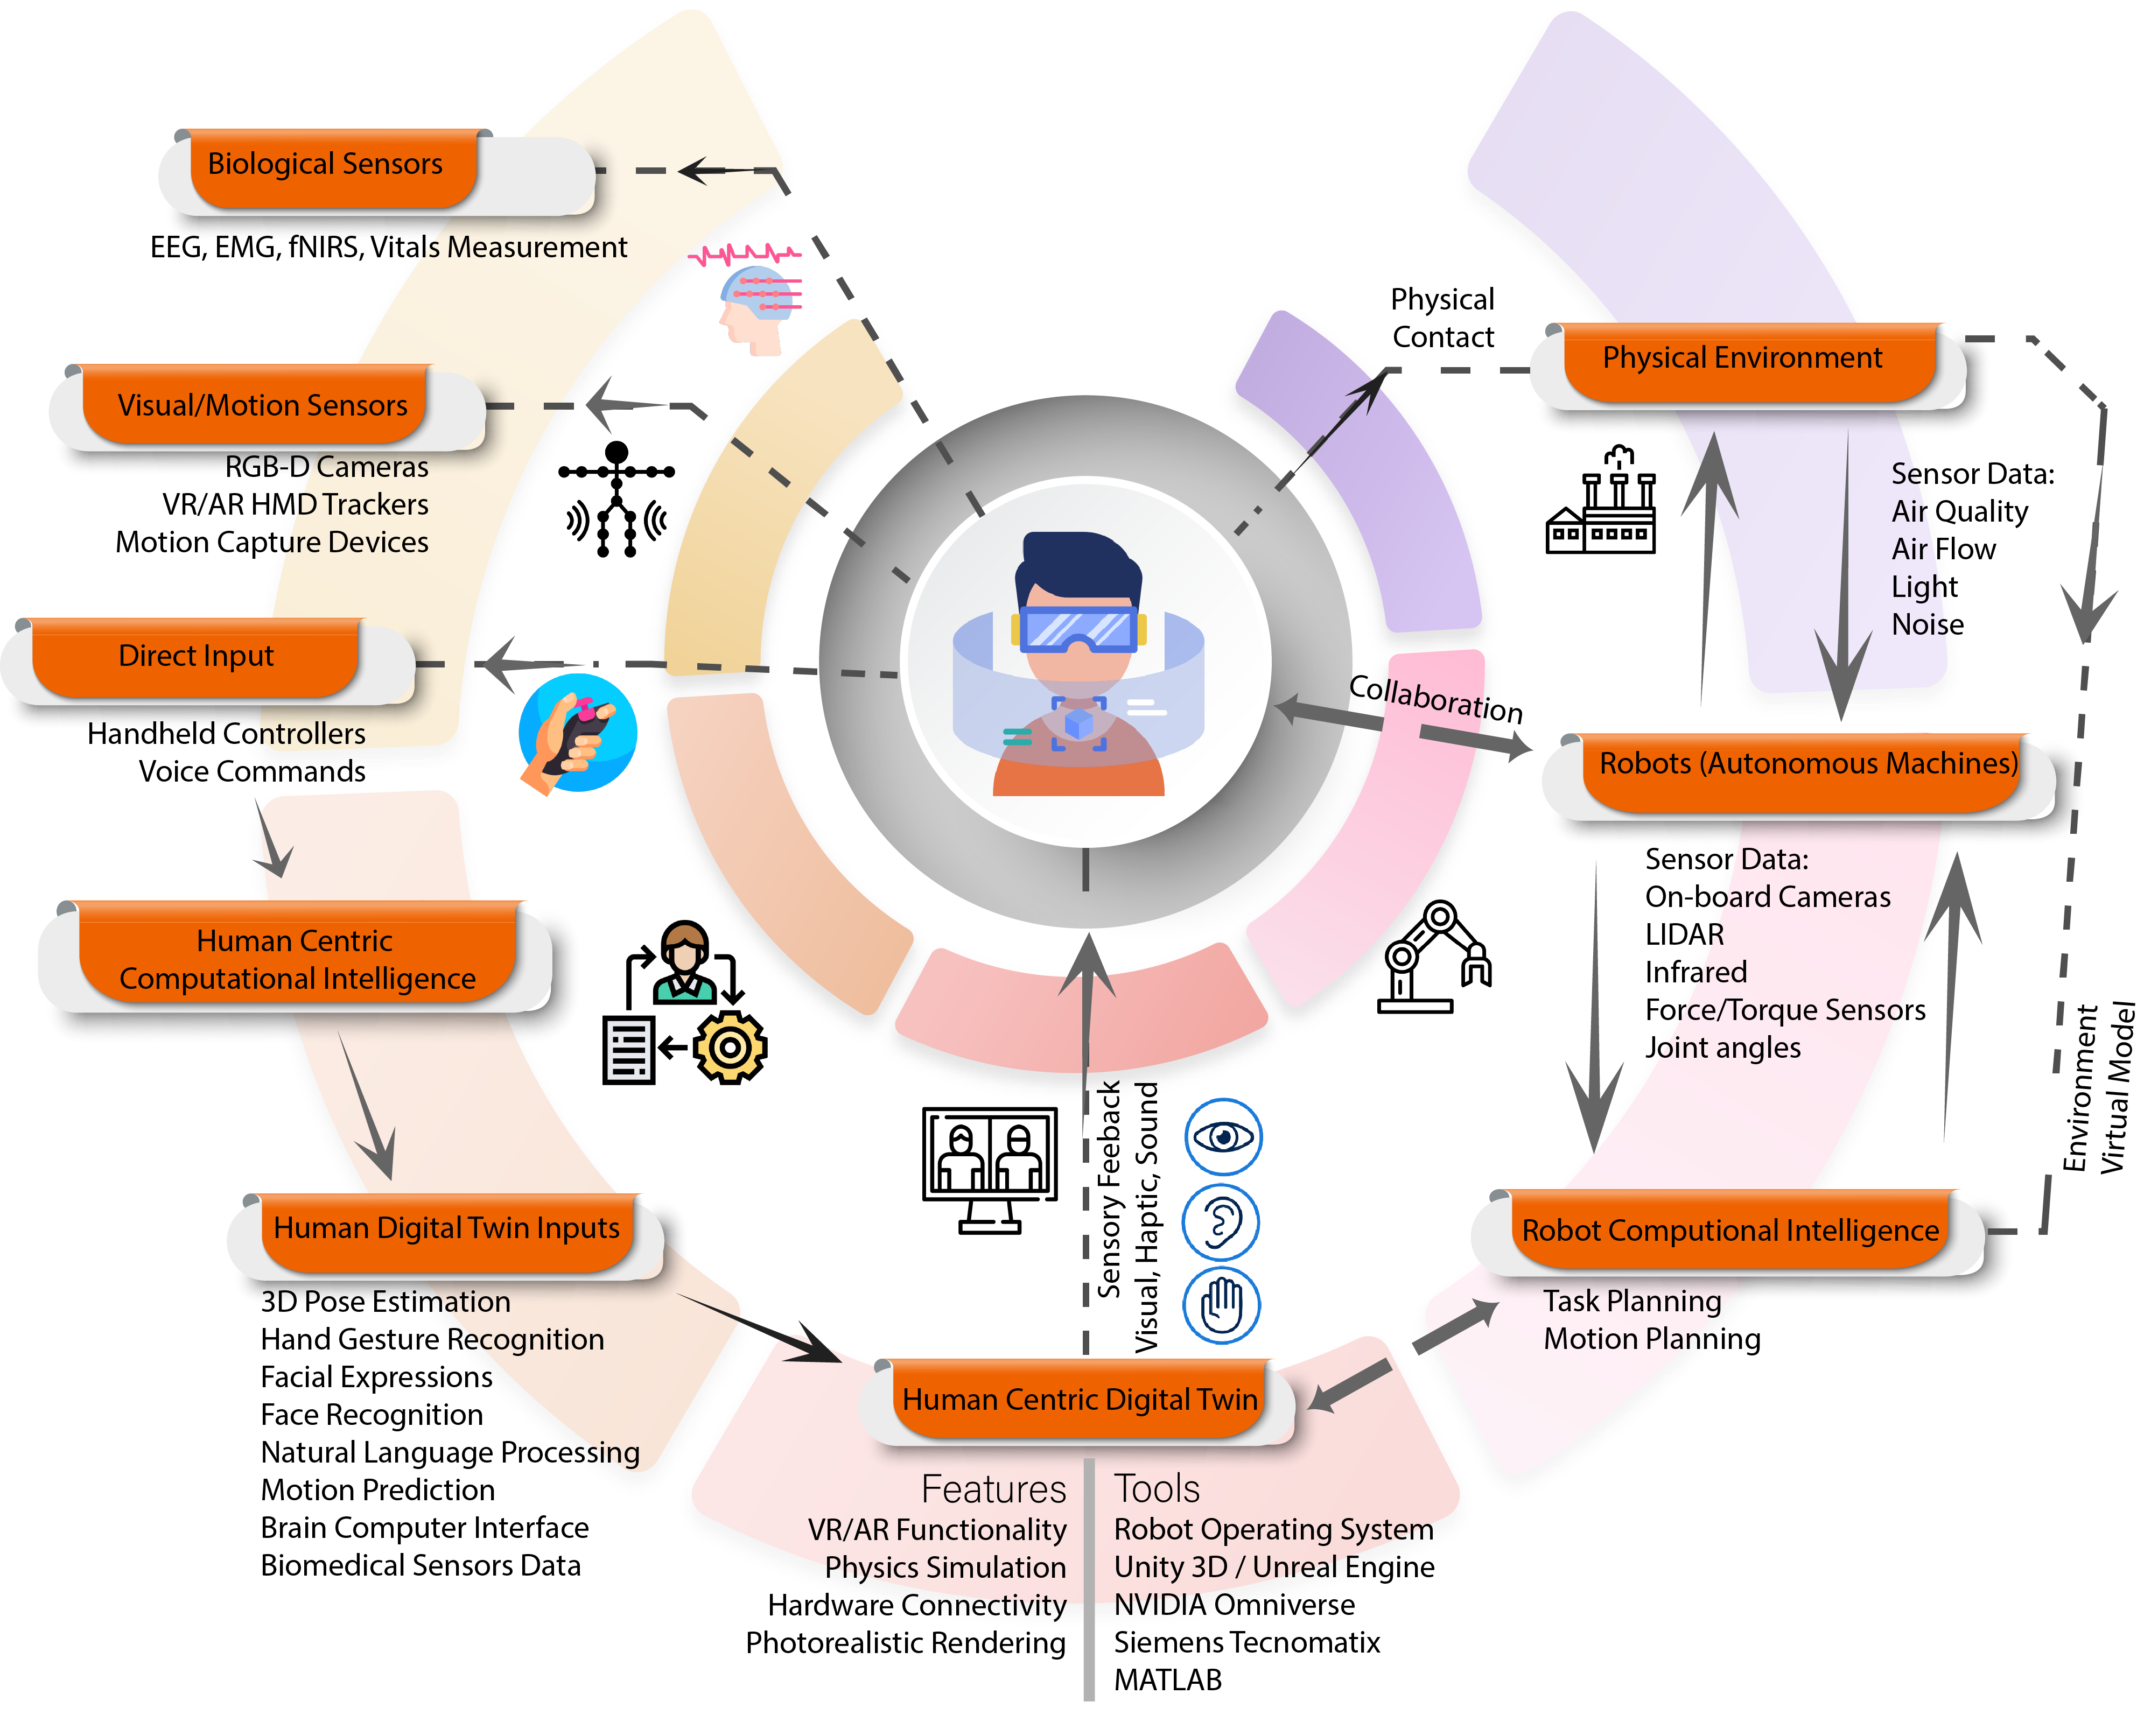
\includegraphics[width=\textwidth]{ThesisFigs/Framework.png}
    \caption{Conceptual overview of the proposed modular framework for Human Intention Prediction based Motion Generation. Information flows from the physical system through the perception and reasoning modules to generate a final motion prediction.}
    \label{fig:framework_overview}
\end{figure}

\subsubsection{Perception and Scene Representation Module}

The Perception and Scene Representation Module serves as the sensory foundation of the framework. It processes raw visual data from cameras to extract meaningful representations of the human operator and the surrounding environment. Key functions include extracting human pose parameters using state-of-the-art human mesh recovery techniques, estimating metric depth to enable 3D scene understanding, tracking human gaze targets to provide cues about operator attention and intent, and converting 2D visual predictions into world-frame 3D coordinates.

\subsubsection{AI-Driven Reasoning and Intent Prediction Module}

The AI-Driven Reasoning and Intent Prediction Module serves as the cognitive core of the framework. It leverages Vision-Language Models (VLMs) to interpret the current task context based on structured task knowledge, predict the current task state and progress within the workflow, forecast future hand positions based on inferred intent, and generate semantic understanding of operator actions and goals. This module bridges the gap between low-level perceptual data and high-level semantic understanding, enabling the system to reason about what the operator is trying to accomplish rather than simply tracking their current pose.

\subsubsection{Human Motion Generation Module}

The Human Motion Generation Module transforms the high-level predictions from the reasoning module into full-body 3D motion trajectories. It employs diffusion-based motion synthesis conditioned on predicted intent, physics-based refinement to ensure motion plausibility, and integration with digital twin visualization for operator feedback. This modularity allows for individual modules to be upgraded as technology advances. While the framework provides the necessary predictive outputs for a complete Human-Centric Digital Twin (HCDT), the implementation of feedback and physical assistance mechanisms is designated as future work.

%----------------------------------------------------------------------------------------
\section{Perception and Scene Representation}
\label{sec:perception_scene}
%----------------------------------------------------------------------------------------

The Perception and Scene Representation module is responsible for extracting structured information from raw visual inputs. This section details the specific techniques employed for human pose estimation, 3D scene understanding, and gaze analysis.

\subsection{Human Pose Representation}

Accurate and expressive human pose representation is fundamental to the framework's ability to understand and predict human motion. This subsection describes the hierarchical approach to pose representation, from the underlying parametric model to the kinematic format used for motion generation.

\subsubsection{SMPL-X Model for Whole-Body Representation}

The framework adopts the Skinned Multi-Person Linear Model with Extensions (SMPL-X) \citep{SMPL-X:2019}, which provides a parametric model for body shape $\boldsymbol{\beta}$, pose $\boldsymbol{\theta}$, and expressive hand and face parameters $\boldsymbol{\psi}$. The SMPL-X model generates a mesh $M(\boldsymbol{\beta}, \boldsymbol{\theta}, \boldsymbol{\psi})$ through a learned blend shape function, enabling realistic representation of human body configurations. The model's differentiable nature allows for gradient-based optimization when fitting to visual observations.

\subsubsection{Global-View Human Mesh Recovery (GVHMR)}

To obtain the pose parameters from monocular RGB video, the framework employs World-Grounded Human Motion Recovery via Gravity-View Coordinates (GVHMR) \citep{multi-hmr2024, gvhmr}. GVHMR reconstructs human pose in a global, gravity-aligned coordinate system, which is essential for the framework as it provides consistent spatial reference across frames, facilitates integration with 3D scene understanding by placing both human and environment in the same coordinate frame, and enables physics-based motion refinement by providing ground-plane alignment. GVHMR outputs the transformation between global and camera coordinates $(R_{wc}, \mathbf{t}_{wc})$, which is used for subsequent 3D scene grounding operations.

\subsubsection{Kinematic Representation for Motion Generation (HumanML3D)}

For kinematic motion generation, the SMPL-X poses are subsequently converted into the representation utilized by HumanML3D \citep{Guo_2022_CVPR}. This format captures frame-relative information such as root angular and linear velocities ($\dot{r}_a, \dot{r}_x, \dot{r}_z$), root height ($r_y$), and local joint positions, rotations, and velocities ($j_p, j_r, j_v$), along with foot contact features ($f$). This relative encoding facilitates the generation of smooth and continuous motions by capturing the dynamics of movement rather than absolute positions.

\subsection{3D Scene Grounding and Contextual Cues}

Beyond human pose estimation, the framework requires understanding of the 3D environment and the operator's attention patterns. This subsection describes the techniques for metric depth estimation and gaze analysis.

\subsubsection{Metric Depth Estimation and World-Frame Conversion}

The module converts the VLM's 2D predictions into 3D world coordinates by combining world-frame human pose reconstruction results and metric depth estimation. Modern monocular depth estimation models, such as Unik3D \citep{unik3d}, provide metric-scale depth predictions from single images.

By leveraging the global-to-camera transformation $(R_{wc}, \mathbf{t}_{wc})$ provided by GVHMR, camera-centric 3D points $\mathbf{x}_c$ can be transformed into a consistent world frame via:
\begin{equation}
    \mathbf{x}_w = R_{wc}^\top (\mathbf{x}_c - \mathbf{t}_{wc})
\end{equation}

This transformation allows any point of interest (POI), such as a tool or a predicted hand location, to be localized in the global reference frame. For specialized applications requiring different or higher-precision grounding, this module can be extended to incorporate other engineered approaches, such as processing fiducial markers or leveraging structured light sensors.

\subsubsection{Human Gaze Target Analysis for Intent Inference}

Human gaze provides a strong cue for immediate intent. Research in cognitive science has established that gaze typically precedes manual action by several hundred milliseconds, making it a valuable predictive signal. A change in the operator's gaze target serves as an indicator of a change in intention, and the location of the gaze target often correlates with the area or object the operator intends to interact with next. Techniques like Gaze-LLE \citep{ryan2024gazelle} can be employed for gaze target tracking to further enrich the context provided to the reasoning and intent prediction module.

%----------------------------------------------------------------------------------------
\section{AI-Driven Reasoning and Intent Prediction}
\label{sec:ai_reasoning}
%----------------------------------------------------------------------------------------

This module serves as the cognitive core of the framework, responsible for interpreting the perceptual data within the context of structured task knowledge and generating predictions about operator intent and future actions.

\subsection{Task Knowledge Representation}

The integration of VLMs for high-level reasoning about tasks and intent requires appropriate data structures to represent task knowledge. This subsection describes the formalisms used and the process for generating task context.

\subsubsection{Directed Acyclic Graphs (DAGs) for Procedural Tasks}

Task dependencies are modeled using formalisms like Directed Acyclic Graphs (DAGs), which define the valid sequence of actions and states within a workflow. Alternative formalisms, such as Planning Domain Definition Language (PDDL) \citep{Singh2023}, Knowledge Graphs (KGs), or Behavior Trees (BTs) \citep{Ahn2022, IEEE-Knowledgebased2021}, can also be integrated depending on application requirements.

\subsubsection{AI-Assisted Generation of Task Context}

For any use case, a common operational flow is followed for establishing task context. Initially, task-specific knowledge, such as assembly instructions, procedural steps, or an example video, is provided to the system. This involves a collaborative effort where an AI model generates an initial draft of a task representation (i.e., the overall goal, a mechanism for state tracking, decomposition into smaller actions, and their dependencies), which is then refined by human experts. This task representation forms a critical part of the context provided to the VLM for prediction.

\subsection{Two-Phase Prediction Pipeline}

The prediction process follows a two-phase approach that decouples long-horizon semantic reasoning from short-horizon spatiotemporal forecasting. This separation allows each phase to be optimized with the most relevant context.

\subsubsection{Phase 1: Task State Prediction}

In the first phase, the VLM analyzes video frames along with appropriate context from the perception module and the task graph. The output is an updated Task State in a structured JSON format, identifying the steps completed, steps in progress, steps available, and the immediate next step. This phase addresses the question of \emph{what} the operator is doing and \emph{where} they are in the overall workflow.

\subsubsection{Phase 2: Future Hand Position Forecasting}

In the second phase, the VLM uses the updated task context along with multimodal data from the perception module to forecast the exact pixel coordinates $(\texttt{x}, \texttt{y})$ for both of the operator's hands at a future time horizon $\Delta t$. This two-phase approach is crucial because it decouples long-horizon semantic reasoning about the overall task from short-horizon spatiotemporal forecasting of immediate motion, allowing each phase to be optimized with the most relevant context. This two-phase pipeline is illustrated in Figure~\ref{fig:prediction_pipeline}.

\begin{figure}[htbp]
    \centering
    \subfloat[Task State Prediction]{
\includegraphics[width=0.48\textwidth, trim=5 0 235pt 0, clip]{ThesisFigs/s5.png}\label{fig:task_state_prediction}}
    \hfill
    \subfloat[Hand Position Forecasting]{
\includegraphics[width=0.48\textwidth, trim=5 0 235pt 0, clip]{ThesisFigs/s6.png}\label{fig:hand_prediction}}
    \caption{The two-phase pipeline of the Reasoning and Intent Prediction Module: (a) In the first phase, the VLM uses the task graph and visual information to update the overall task state. (b) In the second phase, it uses this state along with a sequence of recent frames and additional context to predict the operator's future hand positions.}
    \label{fig:prediction_pipeline}
\end{figure}

\subsection{VLM Prompting Strategies for Intent Prediction}

The effectiveness of VLM-based prediction depends critically on how context is structured and presented. This subsection describes three prompting strategies investigated for optimizing predictive accuracy.

\subsubsection{Baseline: Single-Image Input}

The simplest approach provides only a single current frame to the VLM along with the task graph and state representation. While computationally efficient, this strategy consistently underperforms due to the lack of historical context or ``memory,'' rendering it unable to distinguish between similar visual states that differ in their history. This baseline is evaluated in Chapter~\ref{chap:validation}.

\subsubsection{Rolling Context Window (RCW) for Temporal Analysis}

The Rolling Context Window (RCW) strategy provides the VLM with a window of recent frames (typically 10 frames spaced at 1-second intervals) along with the predicted state from the previous prediction cycle. This approach offers a balance of performance and efficiency, providing temporal context for observing motion patterns while achieving near real-time predictions (2-3 seconds) with efficient models. However, RCW is susceptible to \emph{consistency bias}: if the model erroneously determines a step to be completed, it often fails to revise this belief, causing subsequent predictions to suffer from error propagation.

\subsubsection{In-Context Learning (ICL) with Full Task Examples}

The In-Context Learning strategy provides the VLM with a complete example video of the task along with its corresponding ground-truth state evolution. While ICL achieves the highest accuracy in controlled experiments, the requirement for a large context token count results in significant computational latency and, in some cases, a paradoxical degradation of predictive accuracy due to ``overthinking'' \citep{inversescaling}, thus rendering the approach unsuitable for real-time applications. The trade-offs between these strategies are analyzed in detail in Chapter~\ref{chap:validation}.

%----------------------------------------------------------------------------------------
\section{Human Motion Generation}
\label{sec:motion_generation}
%----------------------------------------------------------------------------------------

As a final, downstream step, the high-level predictions from the Reasoning and Intent Prediction Module drive the Motion Generation Module. This module is crucial for visualizing the predicted intent as a full-body 3D motion and for providing the basis for robot motion planning in collaborative scenarios.

\subsection{Kinematic Motion Synthesis from Intent}

The core of this module adapts diffusion-based motion synthesis techniques to generate plausible future motion conditioned on the predicted intent.

\subsubsection{Adapting the Motion Diffusion Model (MDM)}

The framework builds upon the Human Motion Diffusion Model (MDM) \citep{tevet2023human} and its physics-aware extension CLoSD \citep{tevet2024closd}. The diffusion process operates as follows:

\textbf{Forward Process:} The forward diffusion process $q(x_t|x_{t-1})$ gradually adds Gaussian noise to a motion sequence:
\begin{equation}
    q(x_t|x_{t-1}) = \mathcal{N}(x_t; \sqrt{\alpha_t}x_{t-1},(1-\alpha_t)I)
\end{equation}

where $\alpha_t$ is a noise schedule parameter.

\textbf{Reverse Process:} The reverse process $p_\theta(x_{t-1}|x_t)$ learns to denoise the motion:
\begin{equation}
    p_\theta(x_{t-1}|x_t) = \mathcal{N}(x_{t-1}; \mu_\theta(x_t,t),\sigma_t^2 I)
\end{equation}

The model is trained to minimize an L2 reconstruction loss:
\begin{equation}
    \mathcal{L}_{\text{simple}} = \mathbb{E}_{x_0,t}[\|x_0 - \hat{x}_0\|_2^2]
\end{equation}

\subsubsection{Conditioning on Predicted Task and Target Locations}

The model receives the previous 40 frames of motion data in HumanML3D format and synthesizes future motion sequences for the next two seconds (60 frames at 30 fps). This is additionally conditioned on a textual prompt describing the predicted action or intent, and a target joint (e.g., \texttt{right\_wrist}, \texttt{pelvis}) with its target 3D location derived from the hand position prediction. The Human Motion Model hence synthesizes a physically plausible and semantically guided future motion sequence.

\subsection{Physics-Based Refinement for Plausibility}

Purely kinematic motion synthesis often produces physically implausible results with artifacts such as foot sliding during locomotion, ground penetration or floating, and unnatural joint velocities or accelerations. The CLoSD framework \citep{tevet2024closd} addresses these issues by closing the loop between motion planning and execution. It uses a real-time, autoregressive Diffusion Planner (DiP) to generate kinematic motion plans on-the-fly, which are then executed by a robust reinforcement learning-based tracking controller in a physics simulator. This approach ensures that the final motion respects physical constraints while remaining faithful to the intended action.

\subsection{Visualization in the Digital Twin Environment}

The generated motion sequences are visualized within a virtual representation of the real environment given by a 3D point cloud created by the perception module's depth estimation model. This visualization serves multiple purposes: operators and system designers can visually verify that predictions are reasonable, the digital twin can be used for operator training or for simulating collaborative scenarios, and the predicted human motion provides input for robot motion planning algorithms to ensure safe and efficient collaboration. Figure~\ref{fig:motion_visualization} illustrates sample motion generation results.

\begin{figure}[htbp]
    \centering
    \subfloat[Ground truth motion]{
\includegraphics[width=0.48\textwidth, trim=0 0 0 40, clip]{ThesisFigs/s3.png}}
    \hfill
    \subfloat[Generated motion]{
\includegraphics[width=0.48\textwidth, trim=0 0 0 0, clip]{ThesisFigs/s4.png}}
    \caption{Motion generation visualization: (a) Starting position (red) and ground truth of the human's motion (green) during a manipulation task. (b) Generated motion (blue), with the yellow line representing the target vector for the position of the left wrist.}
    \label{fig:motion_visualization}
\end{figure}

The modularity of the framework also allows for flexible integration of alternative motion visualization methods. For non-real-time applications, AI-driven image-to-video generation tools can synthesize photorealistic visualizations of predicted motion, as illustrated in Figure~\ref{fig:actual_vs_generated}.

\begin{figure}[htbp]
    \centering
    \subfloat[Actual motion frames]{
\includegraphics[width=\linewidth]{ThesisFigs/4cr.png}}
    \vfill
    \subfloat[AI-Generated motion frames]{
\includegraphics[width=\linewidth]{ThesisFigs/5cr.png}}
    \caption{Comparison of actual and AI-generated motion frames for a manipulation task. The AI-generated frames are synthesized using a video generation model conditioned on the starting frame and a text prompt describing the predicted intent.}
    \label{fig:actual_vs_generated}
\end{figure}

%----------------------------------------------------------------------------------------
\section{Chapter Summary}
\label{sec:chapter_summary}
%----------------------------------------------------------------------------------------

This chapter has presented a comprehensive modular framework for context-aware human intention and motion prediction in Human-Centric Digital Twins. The key contributions and design principles can be summarized as follows:

\textbf{Modular Architecture:} The framework is organized into three interconnected modules---Perception and Scene Representation, AI-Driven Reasoning and Intent Prediction, and Human Motion Generation---that work together to transform raw visual observations into full-body 3D motion predictions. This modularity enables independent upgrades and facilitates deployment in resource-constrained environments.

\textbf{Multi-Modal Perception:} The perception module combines state-of-the-art human mesh recovery (GVHMR), metric depth estimation, and gaze tracking to extract rich representations of the operator and environment. The use of gravity-aligned global coordinates enables seamless integration between human pose and scene understanding.

\textbf{Structured Task Knowledge:} The reasoning module leverages Directed Acyclic Graphs and other formalisms to represent procedural task knowledge, enabling the VLM to reason about task state and progress within structured workflows. The AI-assisted generation of task context reduces the burden of manual knowledge engineering.

\textbf{Two-Phase Prediction:} The decoupled prediction pipeline separates long-horizon semantic reasoning (task state prediction) from short-horizon spatiotemporal forecasting (hand position prediction), allowing each phase to be optimized with appropriate context and evaluation metrics.

\textbf{VLM Prompting Strategies:} Three prompting strategies---Single-Image, Rolling Context Window, and In-Context Learning---offer different trade-offs between accuracy, latency, and computational cost. The RCW strategy emerges as a practical choice for near-real-time applications.

\textbf{Physics-Aware Motion Synthesis:} The motion generation module combines diffusion-based synthesis with physics-based refinement to produce full-body motions that are both semantically aligned with predicted intent and physically plausible.

The validation of this framework across diverse use cases and the quantitative analysis of its performance are presented in Chapter~\ref{chap:validation}.